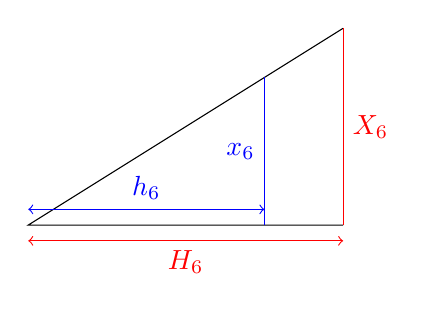
\begin{tikzpicture}

\coordinate (C) at (0, 0);
\coordinate (A) at (4, 0);
\coordinate (B) at (4,2.5);

\draw (A) -- (C) -- (B);
\draw[color = red] (A) -- (B) node[midway, right]{$X_6$};
\draw[color = blue] (3,0) -- (3,1.875) node[midway, left]{$x_6$};
\draw[color = red] [<->] (0,-0.2) -- (4,-0.2) node[midway, below]{$H_6$};
\draw[color = blue] [<->] (0,0.2) -- (3,0.2) node[midway, above]{$h_6$};

\end{tikzpicture}